%-----------------------------------------------------------------------------%
\chapter{\babTiga}
%-----------------------------------------------------------------------------%
%-----------------------------------------------------------------------------%
\section{Tahapan Penelitian}
%-----------------------------------------------------------------------------%
Secara garis besar, tahapan penelitian yang hendak dilaksanakan dalam penelitian ini terdiri dari beberapa tahapan utama yaitu studi literatur, perancangan metode, pengumpulan data, implementasi program, evaluasi dan analisis hasil. Bagan tahapan penelitian dapat dilihat pada \ref{fig:metodologi_penelitian} berikut:

\begin{figure}[htp]
	\centering
	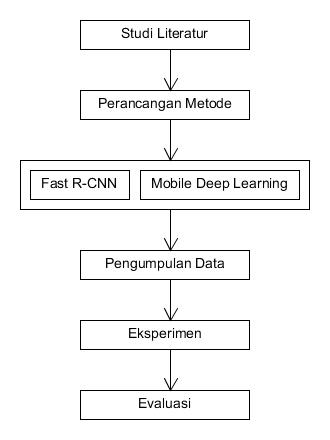
\includegraphics[width=8cm]{pics/metodologi_penelitian}
	\caption{Metodologi penelitian}
	\label{fig:metodologi_penelitian}
\end{figure}

Adapun penjelasan jenis kegiatan yang hendak dilaksanakan adalah sebagai
berikut:
\begin{enumerate}
	\item Studi literatur\\
	Pada tahap ini meliputi pengumpulan berbagai informasi tentang dasar teori serta penelitian-penelitian sebelumnya yang berkaitan dengan penelitian yang akan dilakukan. Tahapan ini bertujuan untuk mengetahui the state of the art dari penelitian yang berkaitan dengan pengenalan convolutional neural network dan deep learning pada teknologi mobile. Hasil kajian tersebut dijadikan sebagai acuan untuk mencari suatu pembaruan terhadap metode yang telah ada.
	\item Perancangan Metode\\
	Pada perancangan metode, ada 2 kegiatan umum yang akan dilakukan yaitu perancangan metode Fast R-CNN untuk melakukan deteksi batik dan metode Mobile Deep Learning untuk melakukan implementasi deep learning pada SoC mobile.
	\item Pengumpulan Data\\
	Pada penelitian menggunakan data batik yang berasal dari penelitian sebelumnya \cite{meta_cnn} dan terdiri dari 5 motif:
	\begin{itemize}
		\item Ceplok
		\item Kawung
		\item Lereng
		\item Nitik
		\item Parang
	\end{itemize}
	\item Eksperimen\\
	Eksperimen berdasarkan rancangan metode yang telah dibuat akan dilakukan menggunakan library Fast R-CNN pada https://github.com/rbgirshick/py-faster-rcnn dan NVIDIA Deep Neural Network library (cuDNN) untuk imeplemntasi pada platform mobile SoC.
	\item Evaluasi dan Analisis Hasil\\
	Pengujian hasil eksperimen meliputi pengujian performa dan akurasi. Selain itu, dalam penelitian ini juga akan dilakukan analisis terhadap waktu komputasi yang dibutuhkan oleh sistem dalam melakukan proses prapengolahan dokumen formulir, segmentasi tulisan dan pengenalan karakter.
\end{enumerate}

\section{Rencana Implementasi}
Secara umum, rencana eksperimen yang akan dilakukan dalam penelitian ini dapat dilihat pada \ref{fig:rencana_implementasi} berikut:
\begin{figure}[htp]
	\centering
	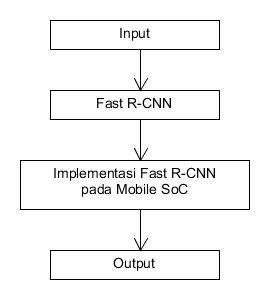
\includegraphics[width=8cm]{pics/rencana_implementasi}
	\caption{Rencana Implementasi}
	\label{fig:rencana_implementasi}
\end{figure}

Berdasarkan gambar \ref{fig:rencana_implementasi}, terdapat dua eksperimen utama yang akan dilakukan pada penelitian ini. Eksperimen pertama fokus kepada implementasi Fast R-CNN untuk pengenalan batik dan pada eksperimen kedua akan fokus kepada integrasi Fast R-CNN dengan DAD dan RLC untuk pengenalan batik pada perangkat mobile. Penjelasan untuk masing-masing proses adalah sebagai berikut:
\begin{enumerate}
	\item Tahap pertama\\
	Tahap pertama akan melakukan implementasi Fast R-CNN untuk mendeteksi batik sesuai dengan arsitektur pada gambar \ref{fig:arsitektur_fcnn}. Arsitektur Fast R-CNN \ref{fig:arsitektur_fcnn} memiliki 2 input yaitu gambar secara utuh dan gambar yang sudah diberikan RoI (Object Proposal). Data input akan diproses kedalam beberapa layer konvolusi dan max pooling untuk mendapatkan feature map. Kemudian untuk setiap gambar yang sudah diberikan RoI atau Object Proposal akan melakukan ekstraksi fitur dari feature map. Tiap vektor fitur akan diproses secara berurutan kedalam Fully Connected Layer dan dibagi ke dalam 2 output layer. Layer pertama menggunakan probabilitas softmax melakukan estimasi pada K kelas object dan kelas background. Layer kedua memberikan 4 output dalam bentuk bilangan real untuk setiap objek kelas K. Untuk setiap 4 nilai dilakukan encoding posisi bounding-box pada salah satu posisi dari kelas K.
	\item Tahap Kedua\\
	Tahap kedua akan berfokus pada implementasi Fast R-CNN dengan integrasi metode DAD dan RLC pada perangkat mobile NVIDIA Tegra K-1 berdasarkan penelitian \cite{deepx}. Implementasi pada perangkat mobile akan mengoptimasi penggunaan sumber daya maupun waktu eksekusi dengan 2 pendekatan:
	\begin{enumerate}
		\item Runtime Layer Compression (RLC)\\
		RLC memiliki 2 komponen utama, komponen pertama melakukan pengurangan dimensi untuk meminimalisir kebutuhan komputasi pada tiap layer. Komponen kedua berfungsi untuk mengatur pengurangan level dimensi yang akan diaplikasikan sebelum model akurasi dipengaruhi pengguna. Input kepada RLC adalah
		\begin{enumerate}
			\item Sepasang adjacent layer ($L$ dan $L + 1$) dari model untuk dieksekusi
			\item Batas error yang digunakan oleh yang menggambarkan observasi dari rekonstruksi error setelah pengurangan dimensi dilakukan
		\end{enumerate}
		2 input tersebut akan disediakan oleh DAD atau merupakan output dari RLS sehingga perubahan matriks bobot antara layer $L$ dan $L+1$ akan membutuhkan parameter dan komputasi yang lebih sedikit.
		\item Deep Architecture Decomposition (DAD)\\
		DAD memiliki 2 komponen diantaranya Decomposition Search dan Recomposition Inference. Komponen pertama bertujuan untuk memperhitungkan proses dekomposisi dari arsitektur deep secara efisien, kemudian dihitung estimasi performa berdasarkan tujuan komputasi. RLC memperluas area pencarian DAD melalui kompresi layer. Komponen kedua akan melakukan inferensi dan memberikan hasil klasifikasi berdasarkan model dengan melakukan rekomposisi dari blok unit yang telah terdekomposisi. Input DAD terdiri dari:
		\begin{enumerate}
			\item Model deep learning yang akan dieksekusi
			\item Kumpulan tujuan performansi
		\end{enumerate}
		DAD akan memberikan output berdasarkan model input dari deep learning.		
	\end{enumerate}
\begin{figure}[htp]
	\centering
	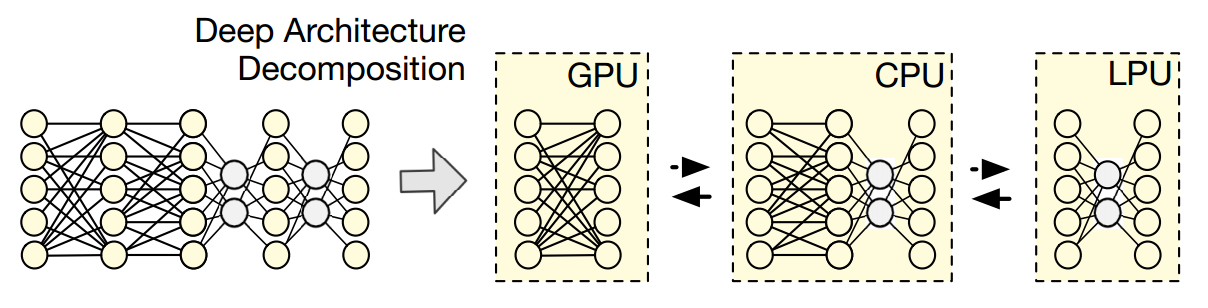
\includegraphics[width=10cm]{pics/dad}
	\caption{Deep Architecture Decomposition}
	\label{fig:dad}
\end{figure}
\end{enumerate}

\section{Jadwal Penelitian}
Penelitian ini diharapkan dapat dilaksanakan tepat waktu sesuai dengan yang telah dijadwalkan. Tabel \ref{tab:timeline_penelitian} akan menampilkan rancangan jadwal penelitian.
\begin{table}
		\centering
	\caption{Timeline penelitian Fast R-CNN pada teknologi mobile}
	\label{tab:timeline_penelitian}
	\begin{tabular}{|l|m{3cm}|l|l|l|l|l|l|l|l|}
		\hline
		No & Deskripsi & Mar-Jun& Jul & Aug & Sep & Oct & Nov & Dec & Jan\\ 
		\hline
		1 & Studi Literatur&x&&&&&&&\\
		\hline
		2 & Seminar Proposal Thesis&&x&&&&&&\\
		\hline
		3 & Pembangunan model Fast R-CNN&&x&&&&&&\\
		\hline
		4 & Implementasi Fast R-CNN&&x&x&&&&&\\
		\hline
		5 & Pembangunan model Fast R-CNN pada mobile&&&&x&&&&\\
		\hline
		6 & Implementasi Fast R-CNN pada mobile&&&&x&x&x&&\\
		\hline
		7 & Evaluasi&&&&&&&x&\\
		\hline
		8 & Sidang Thesis&&&&&&&&x\\
		\hline
	\end{tabular}
\end{table}